\section{Sequence Diagrams}

\begin{figure}[h]
	\centering
	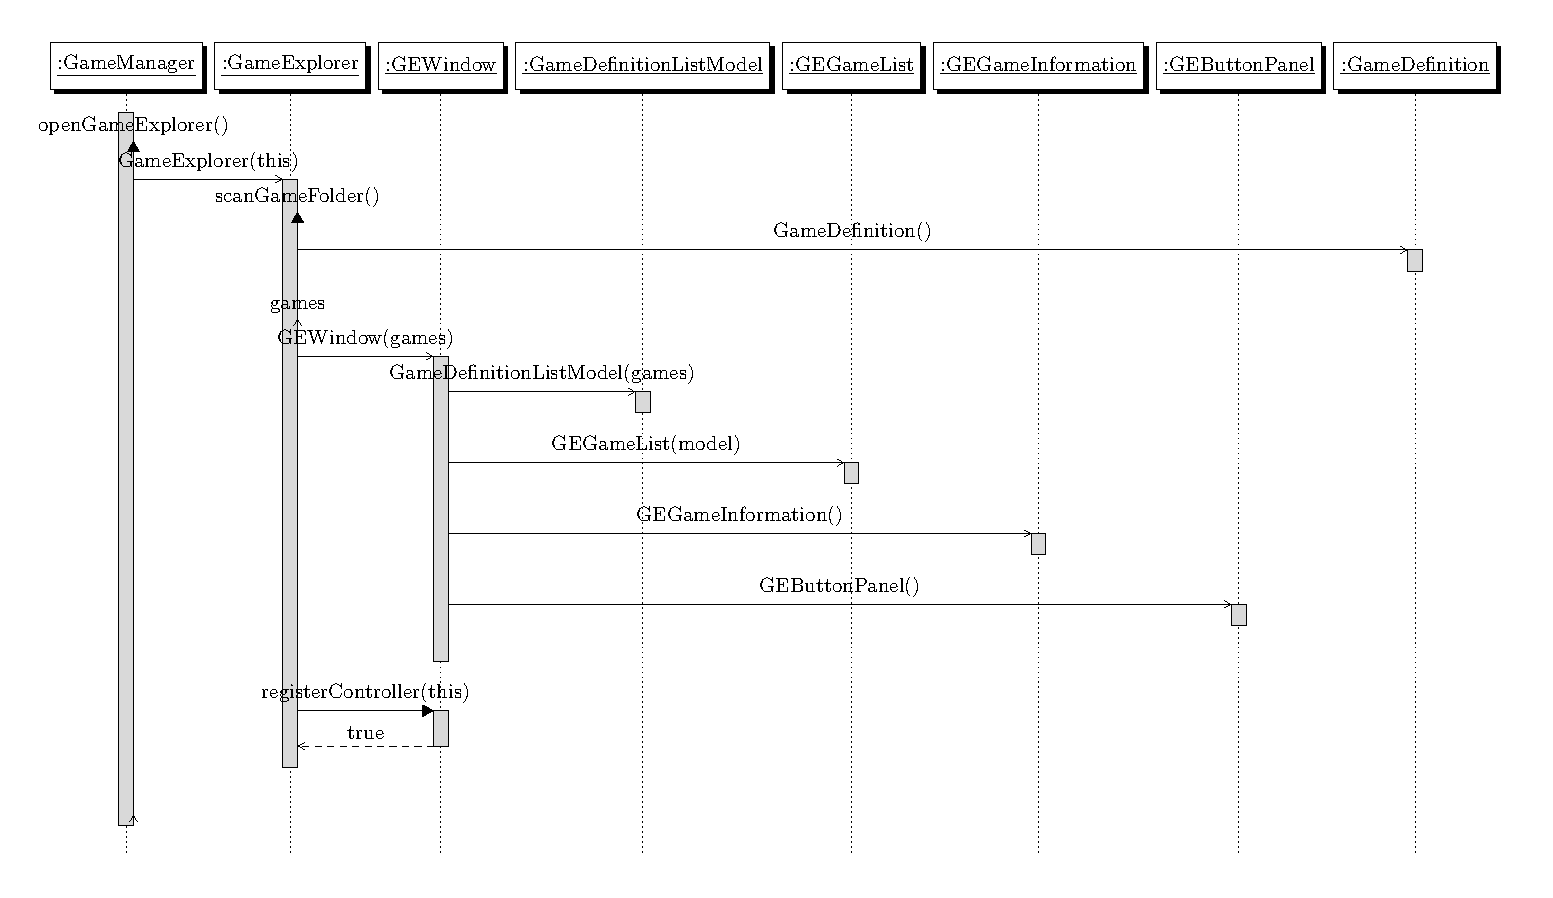
\includegraphics[angle=90,height=0.72\textheight,keepaspectratio]{1-seqGameExplorerInitialization.pdf}
	\caption{Sequence diagram showing the process of initializing the \gameexplorer.}
	\label{img:seqGameExplorerInitialization}
\end{figure}

\begin{figure}[h]
	\centering
	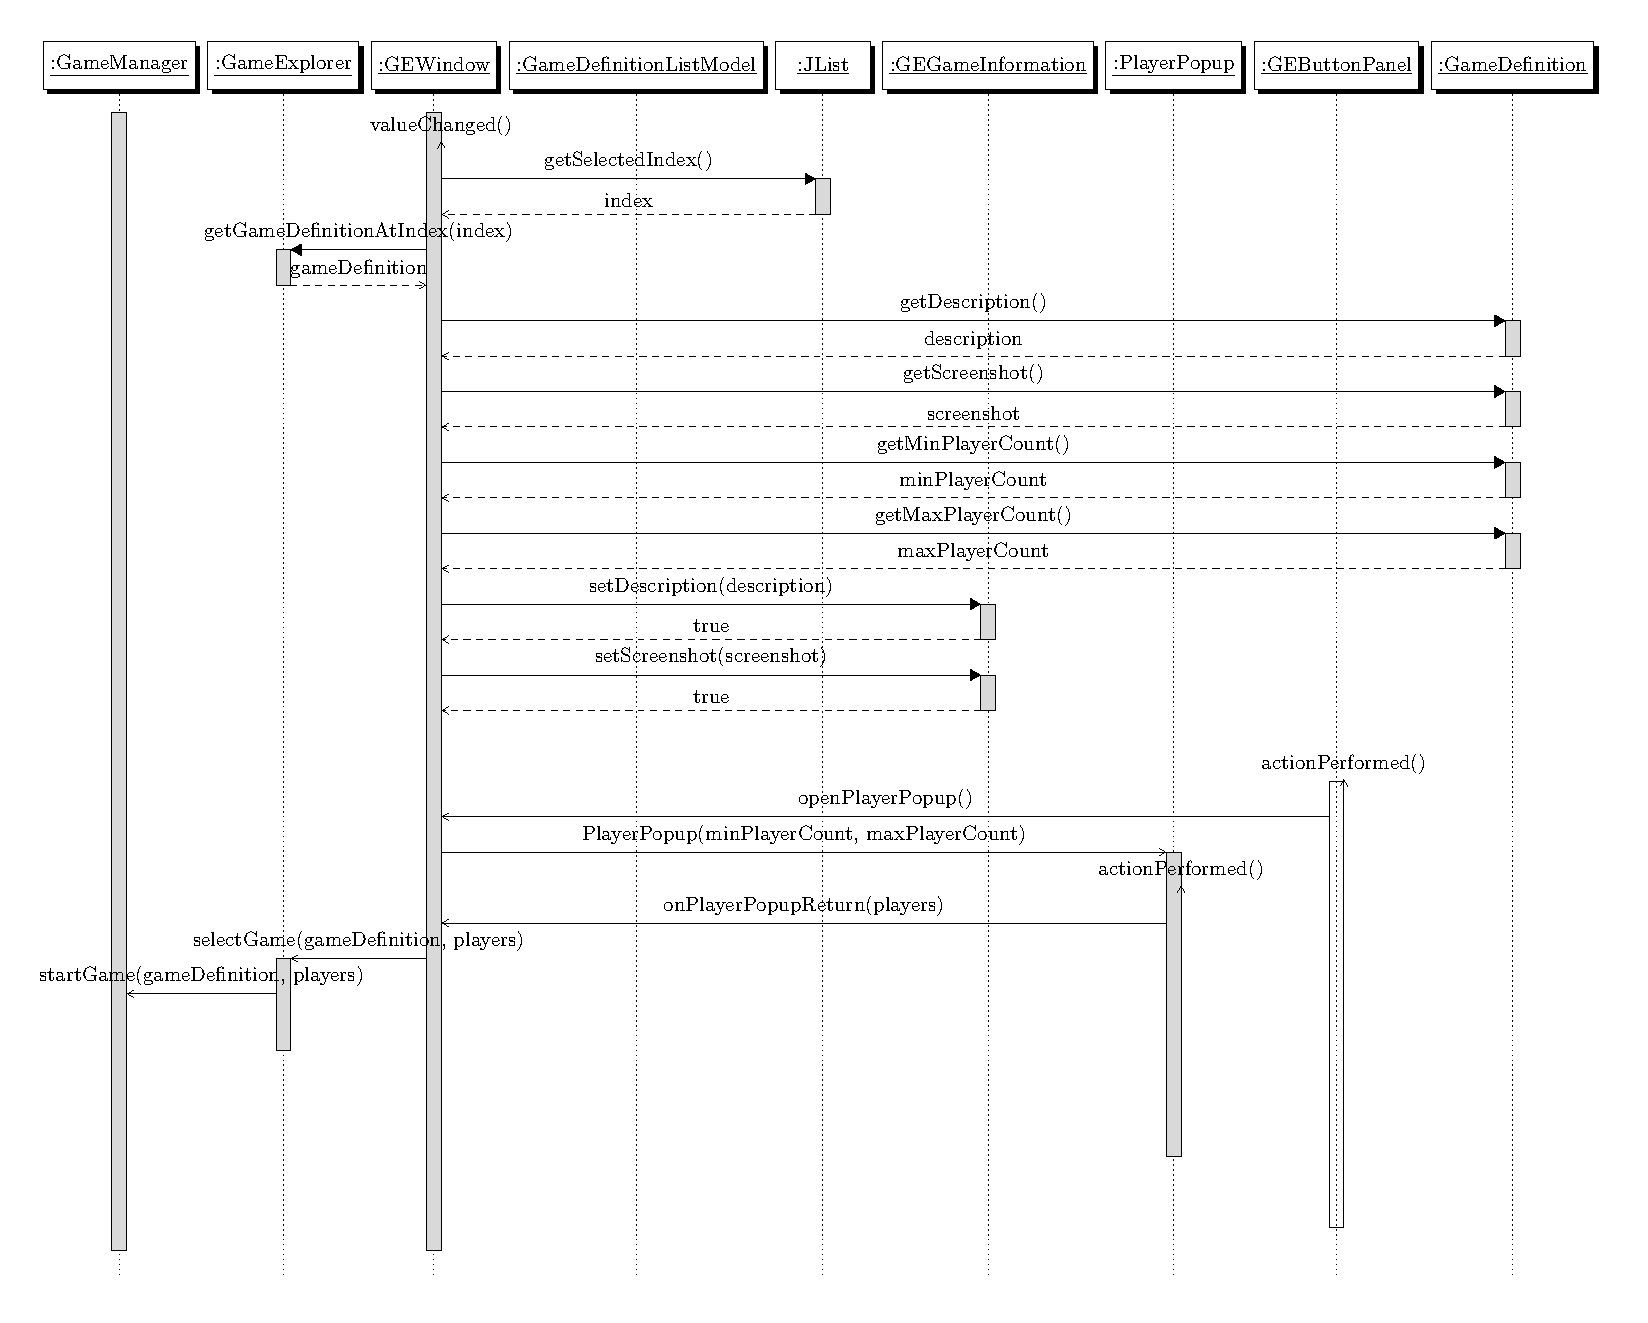
\includegraphics[angle=90,height=0.8\textheight]{2-seqSelectGame.pdf}
	\caption{Sequence diagram showing the process of selecting a game with an initialized \gameexplorer.}
	\label{img:seqSelectGame}
\end{figure}

\begin{figure}[h]
	\centering
	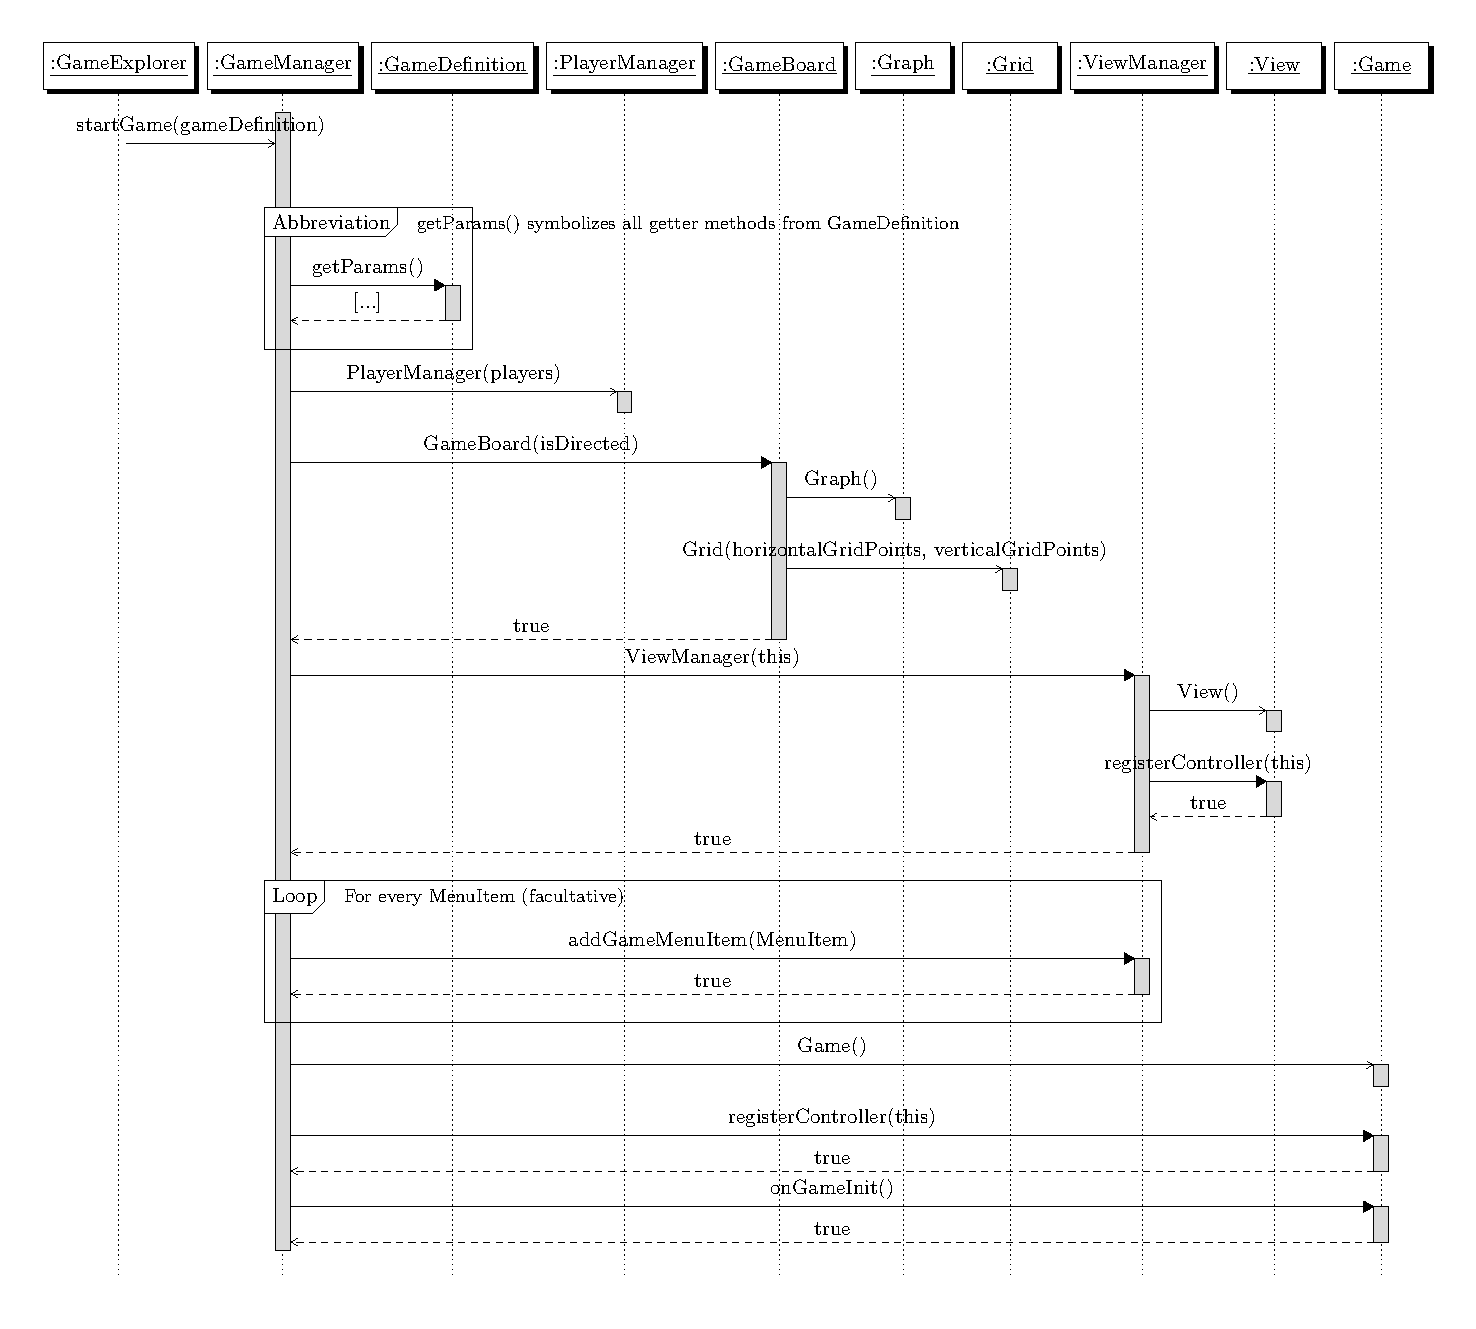
\includegraphics[angle=90,width=1\textwidth]{3-seqGameInitialization.pdf}
	\caption{Sequence diagram showing the process of a game's initialization.}
	\label{img:seqGameInitialization}
\end{figure}

\begin{figure}[h]
	\centering
	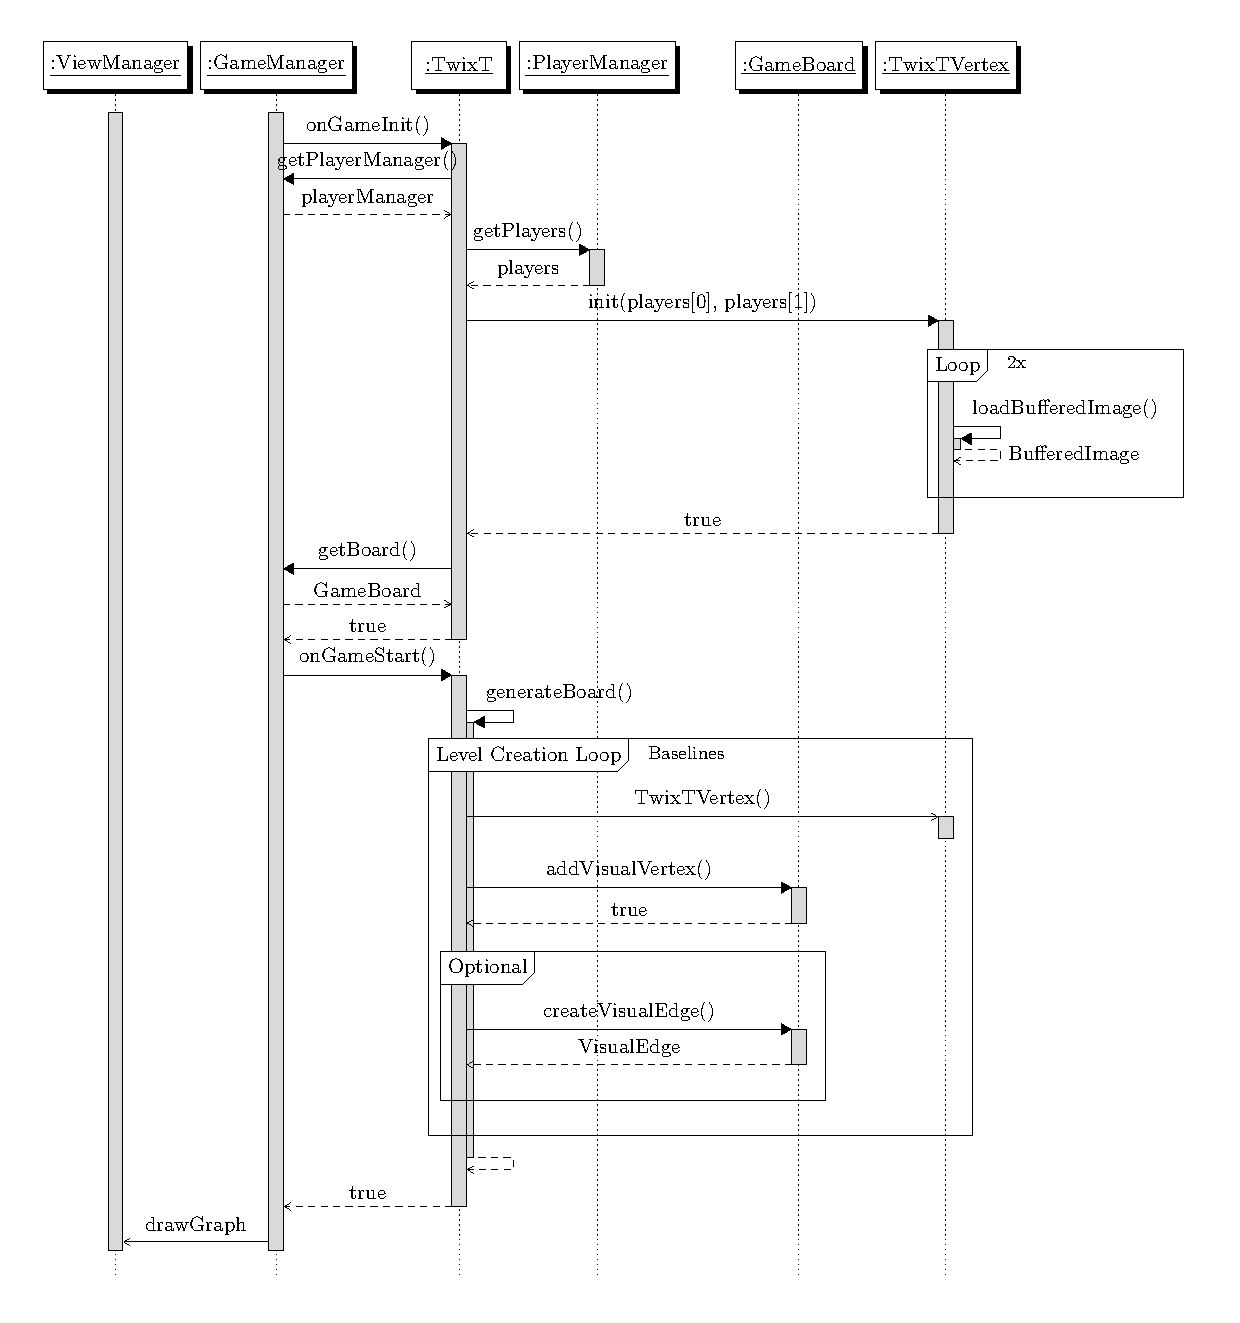
\includegraphics[width=1\textwidth]{4-seqTwixtInitialization.pdf}
	\caption{Sequence diagram showing the process of initializing a new \twixt game.}
	\label{img:seqTwixtInitialization}
\end{figure}

\begin{figure}[h]
	\centering
	\includegraphics[page=2,angle=90,width=1\textwidth]{5-seqTwixt.pdf}
	\caption{Sequence diagram showing the process of creating vertices and edges in the game implementation \twixt.}
	\label{img:seqTwixt}
\end{figure}

\begin{figure}[h]
	\centering
	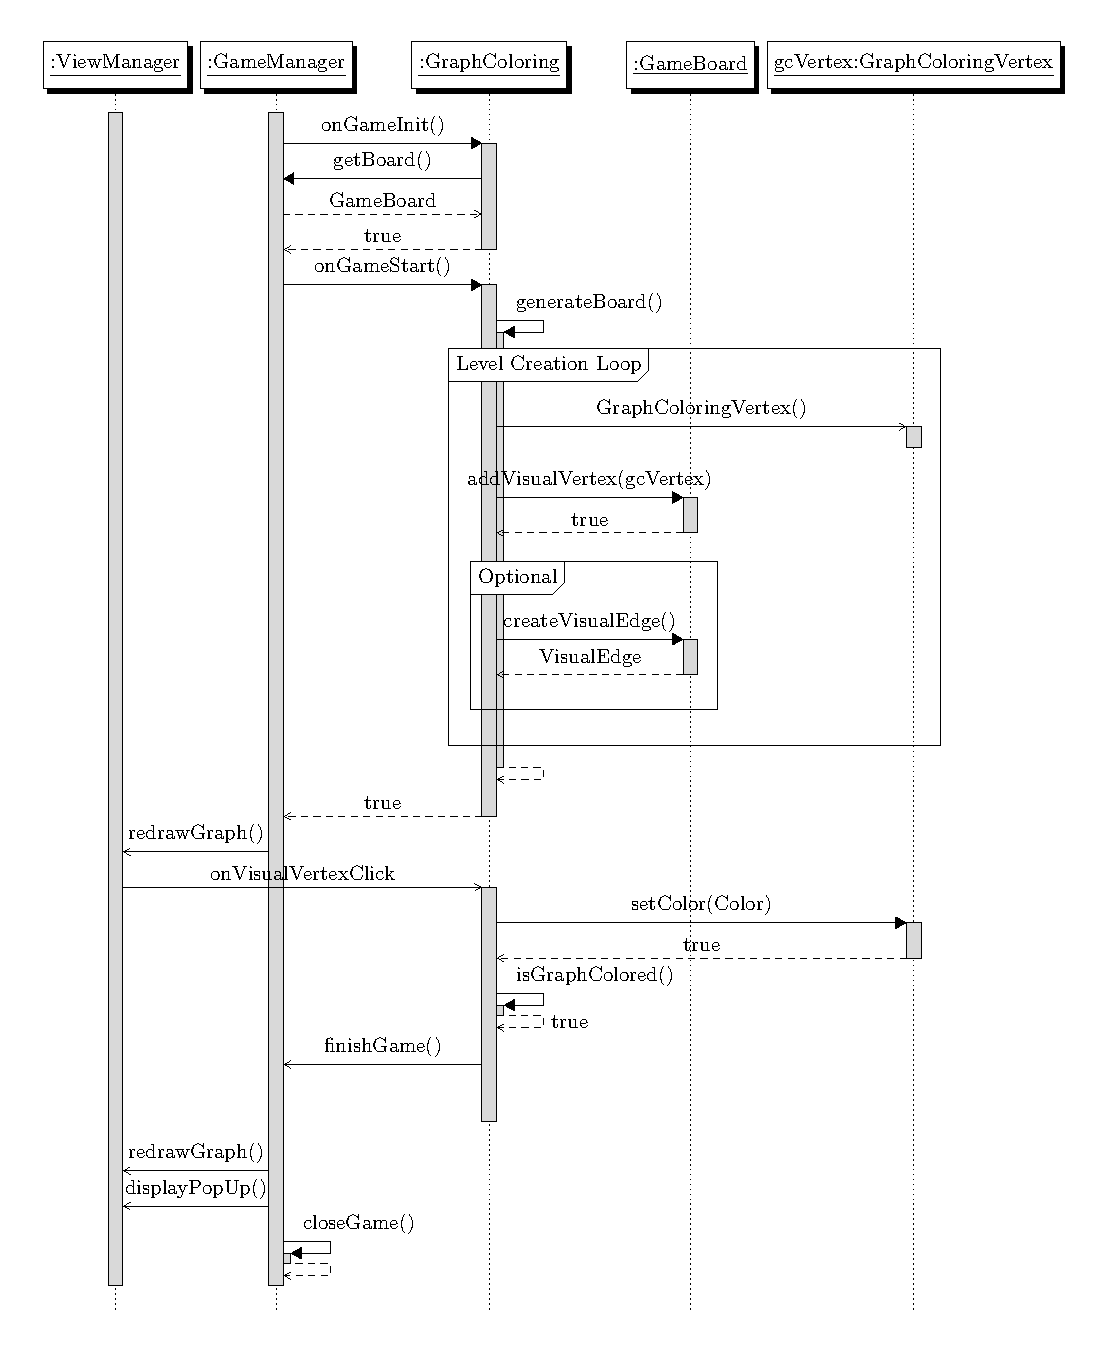
\includegraphics[width=1\textwidth]{6-seqGraphcoloringInitialization.pdf}
	\caption{Sequence diagram showing the process of initializing, playing and winning a \graphcoloring game.}
	\label{img:seqGraphcoloringInitialization}
\end{figure}

\begin{figure}[h]
	\centering
	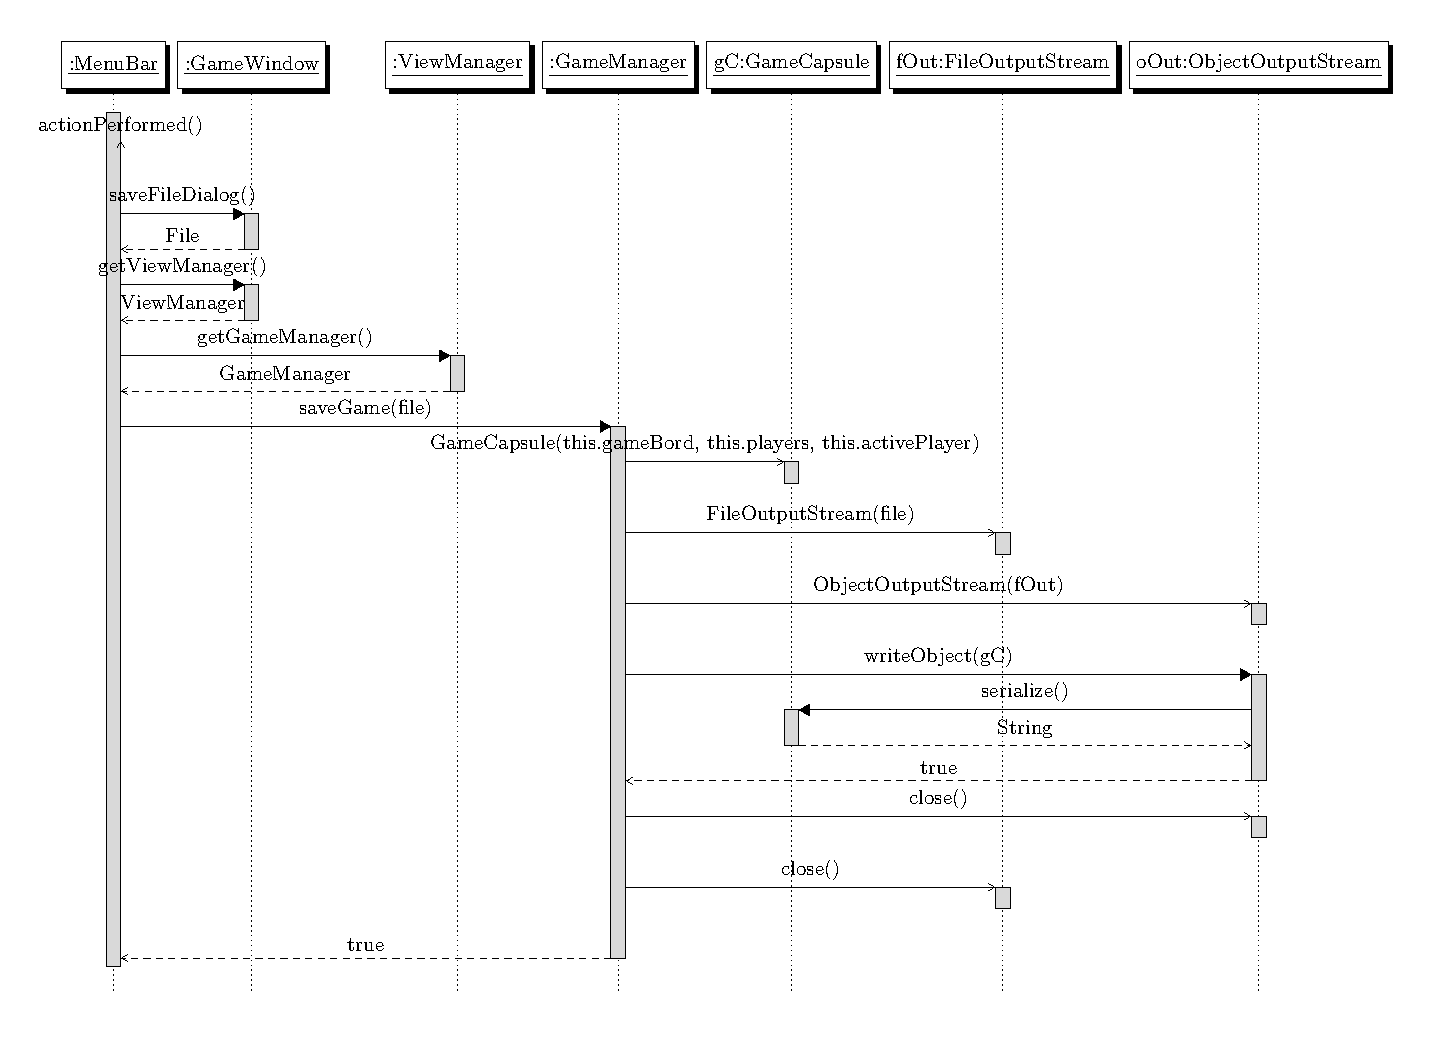
\includegraphics[angle=90,width=1\textwidth]{7-seqSaveGame.pdf}
	\caption{Sequence diagram showing the process of saving a game.}
	\label{img:seqSaveGame}
\end{figure}

\begin{figure}[h]
	\centering
	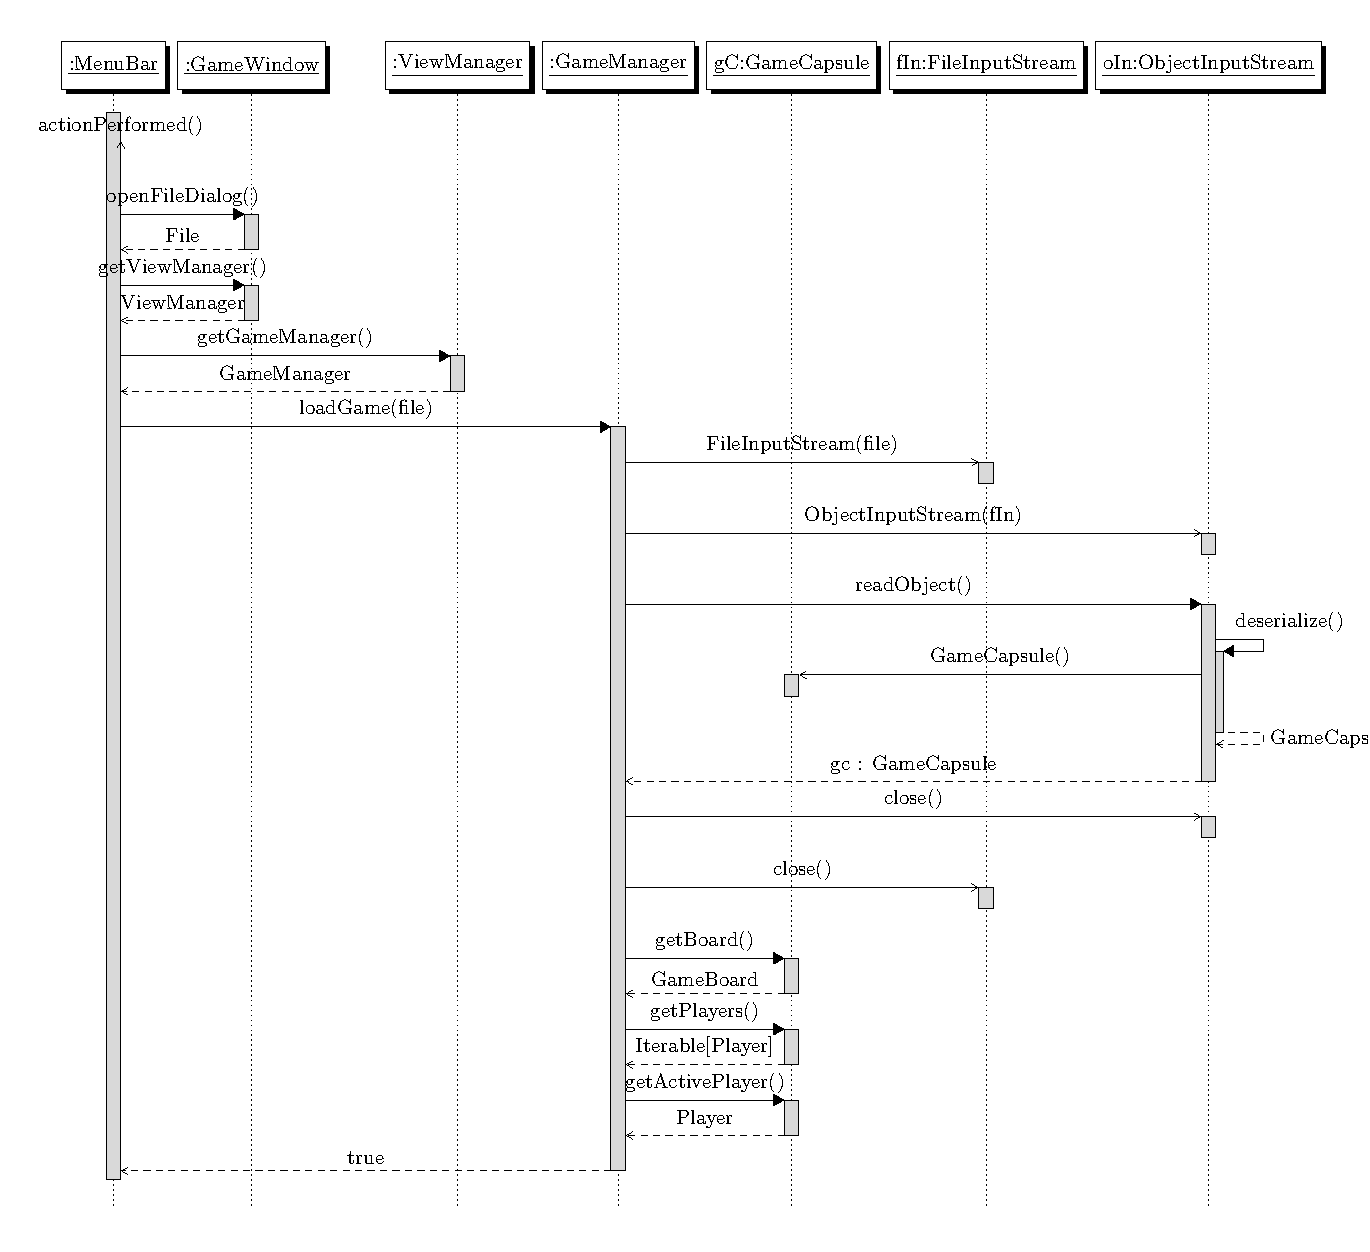
\includegraphics[angle=90,width=1\textwidth]{8-seqLoadGame.pdf}
	\caption{Sequence diagram showing the process of loading a game.}
	\label{img:seqLoadGame}
\end{figure}

\begin{figure}[h]
	\centering
	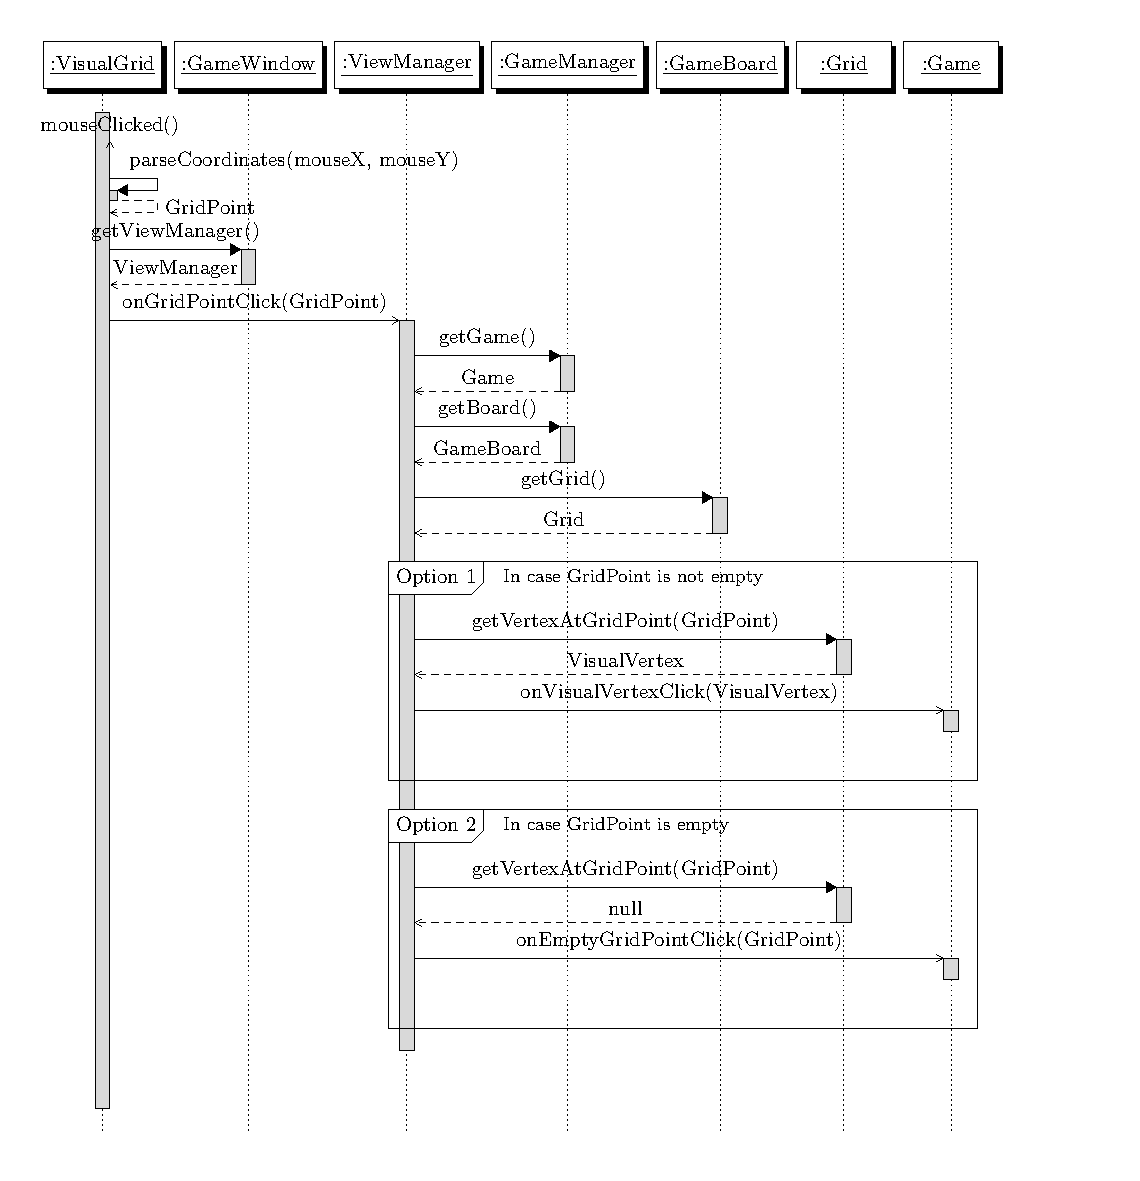
\includegraphics[angle=90,width=1\textwidth]{9-seqClickAction.pdf}
	\caption{Sequence diagram showing the actions performed after a mouse click event.}
	\label{img:seqClickAction}
\end{figure}